\documentclass{llncs}

\usepackage{llncsdoc}
\usepackage{graphicx,url}
\usepackage[brazil]{babel}
\usepackage[utf8]{inputenc}
\usepackage{float}
\usepackage{setspace}

\usepackage{tabularx}
\usepackage{cite}
\usepackage{hyperref}

\begin{document}
\sloppy
\title{Mezuro: Understading source code metrics}

\author{Rafael Manzo\inst{1}, Diego Camarinha\inst{1},
        Dylan Guedes\inst{1}, Paulo Meirelles\inst{1,2}}

\institute{Instituto de Matemática e Estatística -- Universidade de São Paulo (USP)\\
  Rua do Matão, 1010 -- 05508-090 -- Cidade Universitária -- São Paulo -- SP -- Brasil\\
  \email{\{diegoamc,manzo\}@ime.usp.br}
  \and
  Faculdade do Gama -- Universidade de Brasília (UnB)\\
  Gama -- DF -- Brasil\\
  \email{djmgguedes@gmail.com,paulormm@unb.br}}

\maketitle
\begin{abstract}
  % Contexto
  A facilidade de desenvolvimento e manutenção de um software está
diretamente relacionada com a qualidade de seu código-fonte.
  % Problema
  No entanto, analisá-lo impõe dificuldades como, por exemplo, definir as
métricas e interpretar o resultado de uma medição. Além disso, essa prática
ainda não é comum em ambientes de desenvolvimento. Outro problema é a falta de
ferramentas livres que integrem coletores de métricas para diversas liguagens.
  % Soluções propostas
  Neste artigo, apresentamos o Mezuro, uma plataforma web livre para a
avaliação colaborativa de código-fonte. O projeto fornece um meio para comparar
projetos e compartilhar conhecimento sobre métricas, ensinando a configurá-las
e interpretá-las. A plataforma foi idealizada de forma que seja possível
integrar diversos coletores de métricas para diversas linguagens. Atualmente, a
ferramenta permite analisar códigos escritos nas linguagens C, C++, Java e
Ruby.
  % Frase de impacto
  Com este projeto, esperamos disseminar o conhecimento e incentivar o uso de
métricas de código.

\textbf{Palavras-chave:} análise estática, métricas de código-fonte,
\textit{software} livre.
\end{abstract}


\section{Introduction}
\label{sec:intro}

Métricas de código-fonte estático são medidas extraídas a partir das análises
léxica e sintática deste sem compilá-lo ou executá-lo e podem ser primitivas ou
compostas, ou seja, formadas pela composição de uma ou mais métricas
primitivas. Sua principal função é fornecer informações sobre complexidade,
compreensão, testabilidade, manutenibilidade e evolução do
código (REF).

Exemplos de métricas podem ser simples como linhas de código e quantidade de
métodos por classe ou complexas como conexões aferentes de uma classe.  Hoje
existem diversas ferramentas para a simples extração de métricas como
pylint\footnote{\url{http://www.pylint.org/}} (Python),
metric\_fu\footnote{\url{https://github.com/metricfu/metric_fu}} (Ruby) e
Analizo\footnote{\url{http://www.analizo.org/}} (C/C++ e Java), cada uma com
diferentes graus de usabilidade, padrões e conjuntos de métricas, sendo
necessária a criação de uma plataforma que reúna, organize e apresente essas
informações ao usuário, em espcial, no controle da qualidade de um
software durante sua evolução no tempo.

As ferramentas de extração de métricas, em geral, não apresentam uma interface
amigável para seres humanos lerem seus resultados e muito menos um padrão entre
si.  Nesse contexto, este trabalho apresenta a plataforma Mezuro que
(i) possui interface que agrupe as diversas ferramentas disponíveis;
(ii) permita seleção e composição de métricas de forma flexível;
(iii) mantém de um histórico de evolução;
(iv) exibe os resultados de forma amigável;
(v) permite ao usuário a criar seus parâmetros de interpretação conforme um
contexto (por exemplo, linguagem de programação e domínio de aplicação).

\section{Related tools}

Existem duas ferramentas relacionadas com Mezuro. A primeira, o
SonarQube\footnote{\url{http://www.sonarqube.org/}} é um \textit{software}
livre, licenciado como LGPLv3, que oferece uma plataforma de gerenciamento de
qualidade de código. Por meio de \textit{plugins} disponíveis através de uma
biblioteca\footnote{\url{http://docs.codehaus.org/display/SONAR/Plugin+Library/}}.
Em sua versão básica ele classifica problemas encontrados no código e calcula
métricas simples de cobertura de testes e divida técnica em várias linguagens.
Entretanto, seus melhores \textit{plugins} tem código fechado e pago como, por
exemplo, o para análise de
C/C++\footnote{\url{http://www.sonarsource.com/products/plugins/languages/cpp/}}.

A segunda, o Code Climate\footnote{\url{https://codeclimate.com/}} é uma
ferramenta que fornece análise de códigos JavaScript ou Ruby que estejam
disponíveis em um servidor Git. O \textit{software} procura por ``\textit{code
smells}'' no programa do usuário e os classifica como mais ou menos
problemáticos levando em consideração o tamanho dos métodos e duplicação de
blocos. Conforme os encontra, o programa atribui valores ao código para no
final determinar uma nota de \textit{A} a \textit{F} com base no somatório dos
valores encontrados. Note que a análise feita não necessariamente indica um
problema real, uma vez que aquela pode ter sido a implementação escolhida pelo
programador.

Idealizado como uma plataforma de métricas de código, um dos diferenciais do
Mezuro reside na possibilidade de gerar informação sobre o código-fonte de
forma contínua: o usuário decide quando analisar novamente o projeto e
acompanha detalhadamente a evolução das notas ao longo do tempo. Os resultados
de cada análise são públicos, o que permite uma maior transparência entre o
desenvolvedor e a comunidade que utiliza aquele software. Assim, ela
pode decidir se aquela solução atende ou não às suas necessidades e se deve
depositar confiança na qualidade do software desenvolvido.

\section{The Mezuro project}
\label{sec:mezuro}

O Mezuro é dividido em duas partes: processamento e cálculo de métricas de
código-fonte; e a interface gráfica para apresentação dos resultados. Hoje, o
módulo de processamento de é o Kalibro e o módulo de visualização o Prezento,
sendo o Mezuro o projeto inteiro, ou seja, o Kalibro integrado com o Prezento.

Desde a sua primeira implementação em 2010 (REF cbsoft 2012) até a sua
reescrita completa, a arquitetura do sistema evoluiu até a adoção do estilo
arquitetural de micro serviços (REF), para  (i) minimizar a quantidade de
código a ser mantida; (ii) testar e garantir a qualidade do código; (iii)
modularizar a aplicação em diversos serviços independentes.

\begin{figure}[H]
  \centering
    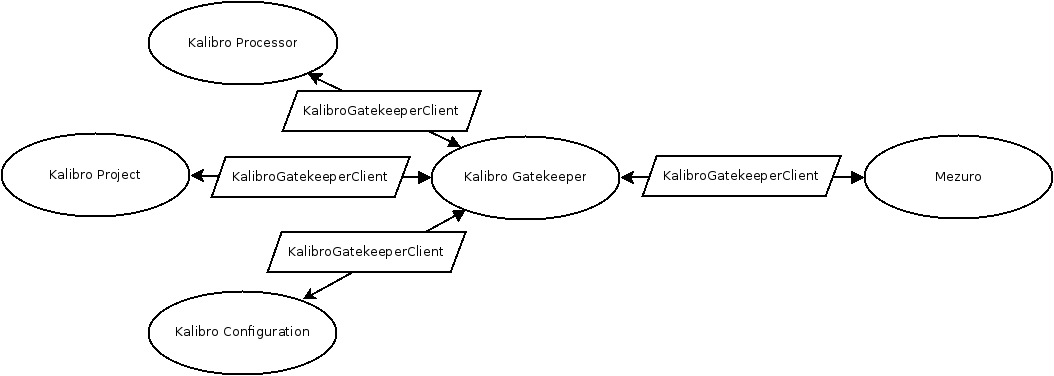
\includegraphics[width=\textwidth]{images/mezuro-architecture-predicted.png}
  \caption{Arquitetura futura do sistema.}
  \label{fig:architecture-2}
\end{figure}

%TODO Dylan: Possivelmente essa figura não é mais do estado atual - ver com o Manzo e Diego.

A Figura \ref{fig:architecture-2} especifica o atual estado do Mezuro. As
elipses são os diferentes softwares envolvidos e os paralelogramos as
interfaces de comunicação entre eles. Na base do Mezuro encontra-se o Kalibro,
segmentado em três entidades menores (...).

No Mezuro, as funcionalidades podem ser divididas em dois grupos:

\begin{itemize}
  \item Projeto
    \begin{itemize}
    \item \textit{Download} do código-fonte a partir de repositórios (Git, Subversion, Bazaar etc) ou via arquivo compactado;
        \item Escolha da periodicidade do processamento do código (1 dia, 2 dias, semanal, quinzenal e mensal);
        \item Escolha de qual configuração de métricas cada repositório irá utilizar;
        \item Nota de cada métrica da configuração para cada arquivo do repositório;
        \item Análise gráfica de cada arquivo do repositório por meio de um gráfico de pontos com notas ao longo do tempo;
        \item Resultados públicos e acessíveis à comunidade.
    \end{itemize}
    \item Configuração
    \begin{itemize}
    \item Criação de configuração e a possibilidade de clonagem;
        \item Estatísticas sobre as configurações mais populares dentro da comunidade;
        \item Criação de intervalos qualitativos associados aos valores das métricas;
        \item Criação de grupos de leitura para a interpretação textual dos resultados das métricas;
        \item Combinações de métricas nativas para criação de análises compostas e mais complexas.
    \end{itemize}
\end{itemize}

%TODO Dylan: Adicionar duas imagens do Mezuro, a lado a lado

O Mezuro tem o formato de uma rede social, no qual os participantes podem ver a
produção de terceiros por meio da avaliação dos projetos ou do clone das
configurações. Essa interação mútua e aberta pode ser interessante para
desenvolvedores, gerentes de projeto, auditores de software e até
mesmo uma equipe de desenvolvimento inteira. O objetivo final é criar uma
comunidade que veja o valor de tais metodologias e como isso pode contribuir
para o sucesso do seu projeto.

\section{Final remarks}

O Mezuro surge como uma potencial resposta para a falta de monitoramento e
padronização de código-fonte e a necessidade de avaliação do mesmo,
considerando que é um \textit{software} livre, altamente customizável, com
suporte para muitas linguagens computacionais, interface amigável, que fornece
histórico de processamentos e também com uma arquitetura planejada para
incorporar novas funcionalidades.

%TODO Paulo: mais coisas ...

\bibliographystyle{splncs03}
\bibliography{mezuro}
\end{document}
